\documentclass[12pt, a4paper]{article}
\usepackage[a4paper, includeheadfoot, mag=1000,
            left=2cm, right=1.5cm, top=1.5cm, bottom=1.5cm,
            headsep=0.8cm, footskip=0.8cm]{geometry}
% Fonts
\usepackage{fontspec, unicode-math}
\setmainfont[Ligatures=TeX]{CMU Serif}
\setmonofont{CMU Typewriter Text}
\usepackage[english, russian]{babel}
% Indent first paragraph
\usepackage{indentfirst}
\setlength{\parskip}{5pt}
% Diagrams
\usepackage{graphicx}
\usepackage{floatrow}
% Python
\usepackage{pythontex}

\begin{document}
\begin{titlepage}

\noindent\textsc{ФГАОУ ВО «Санкт-Петербургский национальный исследовательский
университет информационных технологий, механики и оптики»\\[4mm]
Кафедра физики}
\vfill
\noindent\textbf{РАБОЧИЙ ПРОТОКОЛ И ОТЧЕТ\\[2mm]
ПО ЛАБОРАТОРНОЙ РАБОТЕ №5\\[4mm]
Изучение свободных затухающих электромагнитных колебаний}\\[16mm]
Преподаватель Ефремова Екатерина Александровна\\[2mm]
Студенты Лабушев Тимофей Михайлович, Нестеров Дали Константинович\\[2mm]
Группа P3202
\vfill
\noindent Санкт-Петербург\\[2mm]
2018 г.

\end{titlepage}

\section*{Ход работы}

\subsection*{Исходные параметры}

\begin{pycode}
import numpy as np

L = 10 * 10**-3
C_1 = 0.022 * 10**-6
C_2 = 0.033 * 10**-6
C_3 = 0.047 * 10**-6
C_4 = 0.47 * 10**-6

def r3(f): return np.round(f, 3)
def r2(f): return np.round(f, 2)

T_p = 10**-1 # podgonian
\end{pycode}

\noindent
$$L = \py{L * 10**3} \textup{ мГн} \pm 10\%$$
$$\ C_1 = \py{r3(C_1 * 10**6)} \textup{ мкФ} \pm 10\%
,\ C_2 = \py{r3(C_2 * 10**6)} \textup{ мкФ} \pm 10\%
,\ C_3 = \py{r3(C_3 * 10**6)} \textup{ мкФ} \pm 10\%
,\ C_4 = \py{r3(C_4 * 10**6)} \textup{ мкФ} \pm 10\%$$

\subsection*{Процесс разряда конденсатора}

\begin{pycode}
import re
from tabulate import tabulate

def latex_table(data, headers):
  s = tabulate(data, headers=headers, tablefmt='latex')
  # https://github.com/gregbanks/python-tabulate/issues/5
  s = re.sub(r'(\^\{\})', "^", s); s = re.sub(r'\\([\$\_\{\}\^])', r'\1', s); s = re.sub(r'(\\textbackslash{})', r'\\', s)
  return s
\end{pycode}

\begin{pycode}
from numpy.polynomial.polynomial import polyfit

discharge_resistance_table = [
  [0, 1 * T_p, 48, 17, 5],
  [10, 1 * T_p, 45, 13, 5],
  [20, 1 * T_p, 45, 10, 5],
  [30, 1 * T_p, 44, 8, 5],
  [40, 1 * T_p, 43, 6, 5],
  [50, 1 * T_p, 40, 5, 5],
  [60, 1 * T_p, 39, 9, 3],
  [70, 1 * T_p, 37, 8, 3],
  [80, 1 * T_p, 36, 7, 3],
  [90, 1 * T_p, 34, 6, 3],
  [100, 1 * T_p, 33, 8, 2],
  [200, 1 * T_p, 24, 8, 1],
  [300, 1 * T_p, 17, 3, 1],
  [400, 1 * T_p, 12, 2, 1]
]

def log_decr(n, u0, un):
  return (1 / n) * np.log(u0 / un)
def q_factor(n, u0, un):
  return (2 * np.pi) / (1 - np.exp(-2 * log_decr(n, u0, un)))
def inductance(c, r_m, n, u0, un):
  return (np.pi**2 * c * (r_m + R_0)**2) / log_decr(n, u0, un)**2

def approx_resistance_at_log_decr(l):
  rs_ls = [[r, log_decr(n, u0, un)] for [r, _, u0, un, n] in discharge_resistance_table if r <= 100]
  rs, ls = np.array(rs_ls).T.tolist()
  r_b, r_a = polyfit(ls, rs, 1)
  return r_a*l + r_b

def approx_coeffs_r_l_dependence():
  rs_ls = [[r, log_decr(n, u0, un)] for [r, _, u0, un, n] in discharge_resistance_table if r <= 100]
  rs, ls = np.array(rs_ls).T.tolist()
  return polyfit(rs, ls, 1)

R_0 = -approx_resistance_at_log_decr(0)

def d_log_decr(n, u0, un): return log_decr(n, u0, un) * (1 / u0 + 1 / un)

def d_q_factor(n, u0, un):
  return ((4 * np.exp(2 * log_decr(n, u0, un)) * np.pi) / (-1 + np.exp(2 * log_decr(n, u0, un)))**2) * d_log_decr(n, u0, un)

def d_inductance(r_m, n, u0, un):
  deriv_l = (2*np.pi**2 * C_1 * (r_m + R_0)**2) / log_decr(n, u0, un)**3
  deriv_c = (np.pi**2 * (r_m + R_0)**2) / log_decr(n, u0, un)**2
  return d_log_decr(n, u0, un) * deriv_l + (0.0022 * 10**-6) * deriv_c

table1 = [
  [
    r, t, u0, un, n,
    f'${r2(log_decr(n, u0, un))} \\pm {r2(d_log_decr(n, u0, un))}$',
    f'${r2(q_factor(n, u0, un))} \\pm {r2(d_q_factor(n, u0, un))}$',
    f'${r2(inductance(C_1, r, n, u0, un) * 10**3)} \\pm {r2(d_inductance(r, n, u0, un) * 10**3)}$' if r <= 100 else ''
  ]
  for [r, t, u0, un, n] in discharge_resistance_table
]
\end{pycode}

\py{latex_table(table1, ['$R_{M}$, Ом', '$T$, мс', '$2U_i$, дел', '$2U_{i+n}$, дел', '$n$', '$\\lambda$', '$Q$', '$L$, мГн'])}

Погрешность вычисления логарифмического декремента затухания $\lambda = \frac{1}{n} \ln\frac{U_i}{U_{i+n}}$
с учетом приборных погрешностей находится как:

$$\Delta\lambda = \lambda(\frac{\Delta U}{U_i} + \frac{\Delta U}{U_{i+n}}),\ \Delta U = 1\textup{ дел}$$

Для добротности контура $Q = \frac{2\pi}{1 - e^{-2\lambda}}$ найдем погрешность как:

$$\Delta Q = \frac{\partial Q}{\partial\lambda}\Delta\lambda = \frac{(4e^{2\lambda}\pi)}{(-1 + e^{2\lambda})^2}\Delta\lambda$$

Для индуктивности $L = \frac{\pi^2CR^2}{\lambda^2}$ найдем погрешность как:

$$\Delta L =
  \frac{\partial L}{\partial\lambda}\Delta\lambda +
  \frac{\partial L}{\partial C}\Delta C =
  \frac{2\pi^2 C R^2}{\lambda^3}\Delta\lambda +
  \frac{\pi^2 R^2}{\lambda^2}\Delta C
  ,\ \Delta C = 0.0022 \textup{ мкФ}
$$

\subsection*{Зависимость логарифмического декремента $\lambda$ от сопротивления магазина $R_M$}

\begin{pycode}
import matplotlib.pyplot as plt

l_approx_range = np.arange(0, 400, step=1)
l_b, l_a = approx_coeffs_r_l_dependence()
l_approx = [l_a*r + l_b for r in l_approx_range]

rs, ls = np.array([[r, log_decr(n, u0, un)] for [r, _, u0, un, n] in discharge_resistance_table]).T.tolist()
plt.figure(figsize=(7, 4))
plt.plot(rs, ls, 'o')
plt.plot(l_approx_range, l_approx, '--')
plt.axis((0, 420, 0, 2.1))
plt.grid()
plt.xlabel('Сопротивление магазина $R_m$, Ом', fontsize=12)
plt.ylabel('Логарифмический декремент $\lambda$', fontsize=12)
plt.savefig('rl_plot.pdf', bbox_inches='tight')
\end{pycode}

\begin{figure}[H]
\includegraphics[width=0.8\textwidth]{rl_plot.pdf}
\end{figure}

\subsection*{Индуктивность контура $L$}

Определим собственное сопротивление контура $R_0$ как модуль абсциссы точки с $\lambda = 0$
аппроксимирующей прямой $\lambda(R_M)$:

$$R_0 = \py{r2(R_0)} \textup{ Ом}$$

Считая полное сопротивление контура $R = R_0 + R_M$, вычислим значение индуктивности
контура $L$ для малых значений сопротивления магазина $R_M \leq 100 \textup{ Ом}$ как:

$$L = \frac{\pi^2 C R^2}{l^2}$$

Усредним полученные результаты:

\begin{pycode}
l_table = [
  [inductance(C_1, r, n, u0, un), d_inductance(r, n, u0, un)]
  for [r, _, u0, un, n] in discharge_resistance_table
  if r <= 100
]
L_mean = np.mean(np.array(l_table)[:, 0])
d_L_mean = np.mean(np.array(l_table)[:, 1])
\end{pycode}

$$L_\textup{ср} = \py{r3(L_mean * 10**3)} \pm \py{r3(d_L_mean * 10**3)} \textup{ мГн}$$

\subsection*{Зависимость добротности контура $Q$ от его сопротивления $R$}

\begin{pycode}
rs, qs = np.array([[r + R_0, q_factor(n, u0, un)] for [r, _, u0, un, n] in discharge_resistance_table]).T.tolist()
plt.figure(figsize=(7, 4))
plt.plot(rs, qs, '-o')
plt.axis((0, 450, 0, 20))
plt.grid()
plt.xlabel('Сопротивление контура $R$, Ом', fontsize=12)
plt.ylabel('Добротность контура $Q$', fontsize=12)
plt.savefig('rq_plot.pdf', bbox_inches='tight')
\end{pycode}

\begin{figure}[H]
\includegraphics[width=0.8\textwidth]{rq_plot.pdf}
\end{figure}

\subsection*{Период колебаний контура}

Найдем период колебаний в контуре при минимальном сопротивлении магазина
$R_M = 0 \textup{ Ом},\ R = R_0 = \py{r2(R_0)} \textup{ Ом}$ как: 

\begin{pycode}
def period(r, l, c): return (np.pi * 2) / np.sqrt((1 / (l * c)) - (r**2 / (4 * l**2)))

T_0 = period(R_0, L, C_1)
\end{pycode}

$$T = \frac{2\pi}{\sqrt{\frac{1}{LC} - \frac{R^2}{4L^2}}} = \py{r2(T_0 * 10**3)}$$

\subsection*{Периодичность}

При значении сопротивления магазина $R_M = 500 \textup{ Ом}$ периодичность процесса
разряда конденсатора исчезает. Оценим критическое сопротивление как $R = R_0 + R_M =
\py{r2(R_0 + 500)} \textup{ Ом}$.

Расчетное критическое сопротивление равно
$R_\textup{к} = 2 \sqrt{\frac{L}{C}} = \py{r2(2 * np.sqrt(L / C_1))} \textup{ Ом}$

\subsection*{Сдвиг фаз}

Временной сдвиг между точками графиков тока и напряжения, соответствующих одинаковой
фазе колебаний, $\Delta t = 0.3 \textup{ мс}$. Период $T = 1 \textup{ мс}$.

Вычислим сдвиг фаз между током в контуре и напряжением на конденсаторе как:

\begin{pycode}
delta_e = np.pi - 2*np.pi*(0.3 / 1)
\end{pycode}

$$\delta_{\textup{э}} = \pi - 2\pi \frac{\Delta t}{T} = \py{r3(delta_e)}$$

Выразим сдвиг фаз из циклической частоты колебаний конутра:

$$\delta_{\textup{т}} = \arcsin{\frac{\omega}{\omega_0}}
,\ \omega_0 = \frac{1}{\sqrt{LC}},\ \omega = \sqrt{\omega_0^2 - \beta^2}
,\ \beta = \frac{R}{2L},\ R = R_0 + R_M = \py{r2(R_0 + 100)} \textup{ Ом}$$

\begin{pycode}
def delta_t():
  w_0 = 1 / np.sqrt(L * C_1)
  beta = (R_0 + 100) / (2 * L)
  w = np.sqrt(w_0**2 - beta**2)
  return np.arcsin(w / w_0)
\end{pycode}

\noindent
$$\delta_{\textup{т}} = \py{r3(delta_t())}$$

\subsection*{Период колебаний и емкость конденсатора}

\begin{pycode}
capacitance_period = [
  [0.022 * 10**-6, 1 * T_p],
  [0.033 * 10**-6, 1.2 * T_p],
  [0.047 * 10**-6, 1.3 * T_p],
  [0.47 * 10**-6, 4.2 * T_p]
]

table2 = [
  [c * 10**6, t, r3(period(R_0, L_mean, c) * 10**3), r2(abs(100 * (t - period(R_0, L_mean, c)*10**3) / (period(R_0, L_mean, c)*10**3)))]
  for [c, t] in capacitance_period
]

def period_thomson(c): return 2*np.pi*np.sqrt(L_mean * c)

def table_t_row(c):
  t_th = period_thomson(c)
  t_t = period(R_0, L_mean, c)
  delta = abs(100 * (t_t - t_th) / t_t)
  return [c * 10**6, r3(t_t * 10**3), r3(t_th * 10**3), r2(delta)]

table_t = [table_t_row(c) for [c, _] in capacitance_period]
\end{pycode}

\py{latex_table(table2, ['$C$, мкФ', '$T_{\\textup{э}}$, мс', '$T_{\\textup{т}}$, мс', '$\\delta T$, %'])}

Найдем отклонение вычисленного значения периода $T_\textup{т} = 2\pi / \sqrt{\frac{1}{LC} - \frac{R^2}{4L^2}}$
от экспериментального как:
$$\delta T = 100\% \cdot |\frac{T_\textup{э} - T_\textup{т}}{T_\textup{т}}|$$

При использовании формулы Томсона ($T = 2\pi\sqrt{LC}$) получаются следующие значения:

\py{latex_table(table_t, ['$C$, мкФ', '$T_{\\textup{т}}$, мс', '$T_{\\textup{томс}}$, мс', '$\\delta T_\\textup{т-томс}$, %'])}

\subsection*{Зависимость периода колебаний $T$ от емкости конденсатора $C$}

\begin{pycode}
cs, t1s, t2s = np.array([[c, t1, t2] for [c, t1, t2, _] in table2]).T.tolist()
plt.figure(figsize=(7, 4))
plt.plot(cs, t1s, '-o', label='$T_{э}$')
plt.plot(cs, t2s, '-o', label='$T_{т}$')
#plt.axis((0, 0.5, 0, 0.5))
plt.grid()
plt.legend()
plt.xlabel('Емкость конденсатора $C$, мкФ', fontsize=12)
plt.ylabel('Период колебаний $T$, мс', fontsize=12)
plt.savefig('ct_plot.pdf', bbox_inches='tight')
\end{pycode}

\begin{figure}[H]
\includegraphics[width=0.8\textwidth]{ct_plot.pdf}
\end{figure}

\subsection*{Картина затухающих колебаний}

\begin{figure}[H]
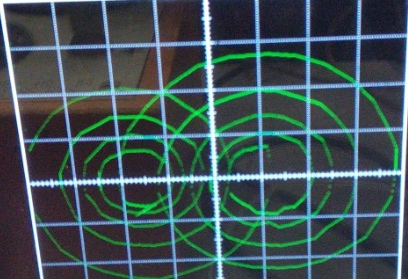
\includegraphics[width=0.6\textwidth]{damping}
\end{figure}

Масштаб $U/\textup{дел}$ по $X$: 1В, $U/\textup{дел}$ по $Y$: 50мВ.

\end{document}
